\documentclass[11pt,]{article}
\usepackage[left=1in,top=1in,right=1in,bottom=1in]{geometry}
\newcommand*{\authorfont}{\fontfamily{phv}\selectfont}
\usepackage[]{mathpazo}


  \usepackage[T1]{fontenc}
  \usepackage[utf8]{inputenc}




\usepackage{abstract}
\renewcommand{\abstractname}{}    % clear the title
\renewcommand{\absnamepos}{empty} % originally center

\renewenvironment{abstract}
 {{%
    \setlength{\leftmargin}{0mm}
    \setlength{\rightmargin}{\leftmargin}%
  }%
  \relax}
 {\endlist}

\makeatletter
\def\@maketitle{%
  \newpage
%  \null
%  \vskip 2em%
%  \begin{center}%
  \let \footnote \thanks
    {\fontsize{18}{20}\selectfont\raggedright  \setlength{\parindent}{0pt} \@title \par}%
}
%\fi
\makeatother




\setcounter{secnumdepth}{0}

\usepackage{color}
\usepackage{fancyvrb}
\newcommand{\VerbBar}{|}
\newcommand{\VERB}{\Verb[commandchars=\\\{\}]}
\DefineVerbatimEnvironment{Highlighting}{Verbatim}{commandchars=\\\{\}}
% Add ',fontsize=\small' for more characters per line
\usepackage{framed}
\definecolor{shadecolor}{RGB}{248,248,248}
\newenvironment{Shaded}{\begin{snugshade}}{\end{snugshade}}
\newcommand{\AlertTok}[1]{\textcolor[rgb]{0.94,0.16,0.16}{#1}}
\newcommand{\AnnotationTok}[1]{\textcolor[rgb]{0.56,0.35,0.01}{\textbf{\textit{#1}}}}
\newcommand{\AttributeTok}[1]{\textcolor[rgb]{0.77,0.63,0.00}{#1}}
\newcommand{\BaseNTok}[1]{\textcolor[rgb]{0.00,0.00,0.81}{#1}}
\newcommand{\BuiltInTok}[1]{#1}
\newcommand{\CharTok}[1]{\textcolor[rgb]{0.31,0.60,0.02}{#1}}
\newcommand{\CommentTok}[1]{\textcolor[rgb]{0.56,0.35,0.01}{\textit{#1}}}
\newcommand{\CommentVarTok}[1]{\textcolor[rgb]{0.56,0.35,0.01}{\textbf{\textit{#1}}}}
\newcommand{\ConstantTok}[1]{\textcolor[rgb]{0.00,0.00,0.00}{#1}}
\newcommand{\ControlFlowTok}[1]{\textcolor[rgb]{0.13,0.29,0.53}{\textbf{#1}}}
\newcommand{\DataTypeTok}[1]{\textcolor[rgb]{0.13,0.29,0.53}{#1}}
\newcommand{\DecValTok}[1]{\textcolor[rgb]{0.00,0.00,0.81}{#1}}
\newcommand{\DocumentationTok}[1]{\textcolor[rgb]{0.56,0.35,0.01}{\textbf{\textit{#1}}}}
\newcommand{\ErrorTok}[1]{\textcolor[rgb]{0.64,0.00,0.00}{\textbf{#1}}}
\newcommand{\ExtensionTok}[1]{#1}
\newcommand{\FloatTok}[1]{\textcolor[rgb]{0.00,0.00,0.81}{#1}}
\newcommand{\FunctionTok}[1]{\textcolor[rgb]{0.00,0.00,0.00}{#1}}
\newcommand{\ImportTok}[1]{#1}
\newcommand{\InformationTok}[1]{\textcolor[rgb]{0.56,0.35,0.01}{\textbf{\textit{#1}}}}
\newcommand{\KeywordTok}[1]{\textcolor[rgb]{0.13,0.29,0.53}{\textbf{#1}}}
\newcommand{\NormalTok}[1]{#1}
\newcommand{\OperatorTok}[1]{\textcolor[rgb]{0.81,0.36,0.00}{\textbf{#1}}}
\newcommand{\OtherTok}[1]{\textcolor[rgb]{0.56,0.35,0.01}{#1}}
\newcommand{\PreprocessorTok}[1]{\textcolor[rgb]{0.56,0.35,0.01}{\textit{#1}}}
\newcommand{\RegionMarkerTok}[1]{#1}
\newcommand{\SpecialCharTok}[1]{\textcolor[rgb]{0.00,0.00,0.00}{#1}}
\newcommand{\SpecialStringTok}[1]{\textcolor[rgb]{0.31,0.60,0.02}{#1}}
\newcommand{\StringTok}[1]{\textcolor[rgb]{0.31,0.60,0.02}{#1}}
\newcommand{\VariableTok}[1]{\textcolor[rgb]{0.00,0.00,0.00}{#1}}
\newcommand{\VerbatimStringTok}[1]{\textcolor[rgb]{0.31,0.60,0.02}{#1}}
\newcommand{\WarningTok}[1]{\textcolor[rgb]{0.56,0.35,0.01}{\textbf{\textit{#1}}}}
\usepackage{longtable,booktabs}

\usepackage{graphicx,grffile}
\makeatletter
\def\maxwidth{\ifdim\Gin@nat@width>\linewidth\linewidth\else\Gin@nat@width\fi}
\def\maxheight{\ifdim\Gin@nat@height>\textheight\textheight\else\Gin@nat@height\fi}
\makeatother
% Scale images if necessary, so that they will not overflow the page
% margins by default, and it is still possible to overwrite the defaults
% using explicit options in \includegraphics[width, height, ...]{}
\setkeys{Gin}{width=\maxwidth,height=\maxheight,keepaspectratio}


\title{Application of Machine Learning on Fundamental Stock Price Analysis  }



\author{\Large Albina Cako, BSc\vspace{0.05in} \newline\normalsize\emph{York University, Certificate in Machine Learning}   \and \Large Colin Green, BSc\vspace{0.05in} \newline\normalsize\emph{York University, Certificate in Machine Learning}   \and \Large Lucy Zhang, BSc\vspace{0.05in} \newline\normalsize\emph{York University, Certificate in Machine Learning}   \and \Large Sean X. Zhang, MSc\vspace{0.05in} \newline\normalsize\emph{York University, Certificate in Machine Learning}  }


\date{}

\usepackage{titlesec}

\titleformat*{\section}{\normalsize\bfseries}
\titleformat*{\subsection}{\normalsize\itshape}
\titleformat*{\subsubsection}{\normalsize\itshape}
\titleformat*{\paragraph}{\normalsize\itshape}
\titleformat*{\subparagraph}{\normalsize\itshape}





\newtheorem{hypothesis}{Hypothesis}
\usepackage{setspace}


% set default figure placement to htbp
\makeatletter
\def\fps@figure{htbp}
\makeatother

\usepackage{hyperref}
\usepackage{graphicx}
\usepackage{subfig}

% move the hyperref stuff down here, after header-includes, to allow for - \usepackage{hyperref}

\makeatletter
\@ifpackageloaded{hyperref}{}{%
\ifxetex
  \PassOptionsToPackage{hyphens}{url}\usepackage[setpagesize=false, % page size defined by xetex
              unicode=false, % unicode breaks when used with xetex
              xetex]{hyperref}
\else
  \PassOptionsToPackage{hyphens}{url}\usepackage[draft,unicode=true]{hyperref}
\fi
}

\@ifpackageloaded{color}{
    \PassOptionsToPackage{usenames,dvipsnames}{color}
}{%
    \usepackage[usenames,dvipsnames]{color}
}
\makeatother
\hypersetup{breaklinks=true,
            bookmarks=true,
            pdfauthor={Albina Cako, BSc (York University, Certificate in Machine Learning) and Colin Green, BSc (York University, Certificate in Machine Learning) and Lucy Zhang, BSc (York University, Certificate in Machine Learning) and Sean X. Zhang, MSc (York University, Certificate in Machine Learning)},
             pdfkeywords = {stock price, fundamental analysis, machine learning, R},  
            pdftitle={Application of Machine Learning on Fundamental Stock Price Analysis},
            colorlinks=true,
            citecolor=blue,
            urlcolor=blue,
            linkcolor=magenta,
            pdfborder={0 0 0}}
\urlstyle{same}  % don't use monospace font for urls

% Add an option for endnotes. -----


% add tightlist ----------
\providecommand{\tightlist}{%
\setlength{\itemsep}{0pt}\setlength{\parskip}{0pt}}

% add some other packages ----------

% \usepackage{multicol}
% This should regulate where figures float
% See: https://tex.stackexchange.com/questions/2275/keeping-tables-figures-close-to-where-they-are-mentioned
\usepackage[section]{placeins}


\begin{document}
	
% \pagenumbering{arabic}% resets `page` counter to 1 
%
% \maketitle

{% \usefont{T1}{pnc}{m}{n}
\setlength{\parindent}{0pt}
\thispagestyle{plain}
{\fontsize{18}{20}\selectfont\raggedright 
\maketitle  % title \par  

}

{
   \vskip 13.5pt\relax \normalsize\fontsize{11}{12} 
\textbf{\authorfont Albina Cako, BSc} \hskip 15pt \emph{\small York University, Certificate in Machine Learning}   \par \textbf{\authorfont Colin Green, BSc} \hskip 15pt \emph{\small York University, Certificate in Machine Learning}   \par \textbf{\authorfont Lucy Zhang, BSc} \hskip 15pt \emph{\small York University, Certificate in Machine Learning}   \par \textbf{\authorfont Sean X. Zhang, MSc} \hskip 15pt \emph{\small York University, Certificate in Machine Learning}   

}

}








\begin{abstract}

    \hbox{\vrule height .2pt width 39.14pc}

    \vskip 8.5pt % \small 

\noindent Abstract:


\vskip 8.5pt \noindent \emph{Keywords}: stock price, fundamental analysis, machine learning, R \par

    \hbox{\vrule height .2pt width 39.14pc}



\end{abstract}


\vskip -8.5pt


 % removetitleabstract

\noindent  

\hypertarget{introduction}{%
\section{Introduction}\label{introduction}}

\hypertarget{background}{%
\subsection{Background}\label{background}}

The stock market is a marketplace where investors can purchase or sell
shares of publicly traded companies. As of 2019, the amount of money
invested in the global stock market has surpassed over \$85 trillion.
Since the inception of the stock market, investors have continuously
sought to develop methods of improving their returns. Currently, there
are two main schools of thought when it comes to stock market analysis:
technical analysis and fundamental analysis.

\emph{Technical analysis} looks at buying and selling trends of a
particular stock. The core theory of technical analysis assumes that all
information is already factored into the stock price. As such, technical
analysis prioritizes identifying patterns or trends in time-series data
to predict stock price at a particular time point.

\emph{Fundamental analysis} attempts to measure the intrinsic value of a
company by studying information from that company's balance sheet, such
as revenue or debt. Fundamental analysis attempts to identify companies
that appear to be `undervalued' or `overvalued' to inform buy or sell
recommendations.

Previous machine learning models that simulated stock market returns
have largely focused on using time series data to predict stock trends,
which is more akin to technical analysis. However, such models have run
into challenges such as overfitting or a lack of interpretability. One
benefit of fundamental analysis is that it allows the investor to learn
about which aspects of a company's financials will influence that
company's stock price; it is more interpretable. As there are dozens to
hundreds of variables on a company's balance sheet, the use of
machine-learning approaches may augment fundamental analysis by
pinpointing important markers of a company's financials and their
relationship with the stock price.

\hypertarget{objective}{%
\subsection{Objective}\label{objective}}

In this project, we apply machine learning and data science techniques
to predict the market capitalization, which is how much company is worth
on the stock market. Stock price can then be calculated by dividing
market capitalization by total number of stocks issued. We also create
an application using R shiny to be used as a guide for investors. This
application would be used individuals interested in checking their stock
analyses with a machine learning prediction. The application could be
used by financial analysts, portfolio managers, or non-professional
investors with an interest in fundamental analysis.

\hypertarget{methodology}{%
\section{Methodology}\label{methodology}}

\hypertarget{data-preprocessing}{%
\subsection{Data Preprocessing}\label{data-preprocessing}}

The original dataset was obtained from Kaggle. Five datasets were
combined together containing stock information for different years:
2014, 2015, 2016, 2017 and 2018, respectively. There were 200 columns in
the dataset, however, after analyzing the data, only 66 columns were
chosen as fundamental columns and were included in the project.

\hypertarget{missingness}{%
\subsection{Missingness}\label{missingness}}

The dataset was assessed for missing values. Any columns that had more
then 1/3 of the data as missing values were removed. For the rest of the
columns, data imputation was performed using the MICE package in R. We
used the CART method to impute the data. CART imputes values by using
classification and regression trees. Four columns were left with missing
values after imputation. Those columns were removed leaving a dataset
with a total of 62 columns.

\hypertarget{feature-selection}{%
\subsection{Feature Selection}\label{feature-selection}}

It is important to note that this project contains both unsupervised and
supervised learning. Decision Tree was used for feature selection.
Feature tree is a classification algorithm used for classification
problems, as well as detecting variable importance in a dataset. The top
10 important variables from the decision tree were selected as the
features. They were used to run k-means unsupervised learning, which
determined 4 clusters of data. Then, supervised learning dataset was
selected as the top 10 variables selected from the decision tree plus
the cluster \# (as a categorical variable) and the Sector of the stock.
Thus, the unsupervised learning data contained 10 features, while the
supervised learning data contained 12.

\begin{longtable}[]{@{}lll@{}}
\caption{Comman Predictor variables}\tabularnewline
\toprule
Variable & & Type\tabularnewline
\midrule
\endfirsthead
\toprule
Variable & & Type\tabularnewline
\midrule
\endhead
Consolidated.Income & & numeric\tabularnewline
Dividend.payments & & numeric\tabularnewline
Stock.based.compensation & & numeric\tabularnewline
Income.Tax.Expense & & numeric\tabularnewline
Retained.earnings deficit & & numeric\tabularnewline
Operating.Cash.Flow & & numeric\tabularnewline
Operating.Expenses & & numeric\tabularnewline
R.D.Expenses & & numeric\tabularnewline
Total.debt & & numeric\tabularnewline
Long.term.debt & & numeric\tabularnewline
\bottomrule
\end{longtable}

\hypertarget{principle-component-analysis}{%
\subsection{Principle Component
Analysis}\label{principle-component-analysis}}

We applied Principle Component Analysis (PCA) to our feature dataset for
dimension reduction before doing unsupervised learning using the k-Means
clustering algorithm. PCA creates orthogonal `principle components' of
the feature set, reducing multicollinearity within the data. Since the
k-means algorithm is non-parametric, reducing multicollinearity before
performing k-Means clustering, could lead to greater discrimination
between the clusters.

\hypertarget{unsupervised-learning}{%
\subsection{Unsupervised Learning}\label{unsupervised-learning}}

The k-Means algorithm was performed in order to cluster the data before
supervised learning. The number of clusters was evaluated by plotting
the within-cluster sum of squares (WSS) against the number of clusters
(k). The optimal number of clusters was chosen based on a combination of
the `elbow method' and domain knowledge.

\hypertarget{supervised-learning}{%
\subsection{Supervised Learning}\label{supervised-learning}}

Supervised learning was performed using four algorithms: XGBoost, Random
Forest, Lasso Model and GBM Model. XGBoost is a very powerful algorithm
which drives fast learning and offers efficient usage of storage.
XGBoost uses ensemble learning, which is a systematic solution that
combines the predictive power of multiple learners. It outputs a single
model that gives the combined output from many models. This allows the
opportunity to not rely on the results of a single machine learning
model.In this particular model, the trees are built sequentially, such
that the next tree focuses on reducing the errors of the previous tree.
Random forest is another supervised learning model that uses
``ensemble'' method to fit many decision trees by using a subset of the
rows and then taking the ``mode'' of the predicted class. GBM, which
stands for Gradient Boosting Machine, is also a gradient boosting
algorithm that works similar to XGBoost. However, XGBoost has more
tuning parameters, thus both algorithms were chosen for comparison. All
models were ran and they were evaluated using the k-fold cross
validation method. Three accuracy metrics: Root Mean-Squared Error
(RMSE), Pearson correlation (\(R^2\)), and Mean Average Error (MAE) were
used to chose the final model.

\hypertarget{deployment}{%
\subsection{Deployment}\label{deployment}}

\hypertarget{results}{%
\section{Results}\label{results}}

\begin{longtable}[]{@{}lll@{}}
\caption{Data Dictionary}\tabularnewline
\toprule
\begin{minipage}[b]{0.19\columnwidth}\raggedright
Variable\strut
\end{minipage} & \begin{minipage}[b]{0.10\columnwidth}\raggedright
\strut
\end{minipage} & \begin{minipage}[b]{0.62\columnwidth}\raggedright
Type\strut
\end{minipage}\tabularnewline
\midrule
\endfirsthead
\toprule
\begin{minipage}[b]{0.19\columnwidth}\raggedright
Variable\strut
\end{minipage} & \begin{minipage}[b]{0.10\columnwidth}\raggedright
\strut
\end{minipage} & \begin{minipage}[b]{0.62\columnwidth}\raggedright
Type\strut
\end{minipage}\tabularnewline
\midrule
\endhead
\begin{minipage}[t]{0.19\columnwidth}\raggedright
X.1\strut
\end{minipage} & \begin{minipage}[t]{0.10\columnwidth}\raggedright
\strut
\end{minipage} & \begin{minipage}[t]{0.62\columnwidth}\raggedright
Index of the records\strut
\end{minipage}\tabularnewline
\begin{minipage}[t]{0.19\columnwidth}\raggedright
X\strut
\end{minipage} & \begin{minipage}[t]{0.10\columnwidth}\raggedright
\strut
\end{minipage} & \begin{minipage}[t]{0.62\columnwidth}\raggedright
Stock ticker symbol\strut
\end{minipage}\tabularnewline
\begin{minipage}[t]{0.19\columnwidth}\raggedright
Consolidated.Income\strut
\end{minipage} & \begin{minipage}[t]{0.10\columnwidth}\raggedright
\strut
\end{minipage} & \begin{minipage}[t]{0.62\columnwidth}\raggedright
Describe all changes in equity except investments made by owners in a
period of time\strut
\end{minipage}\tabularnewline
\begin{minipage}[t]{0.19\columnwidth}\raggedright
Dividend.payments\strut
\end{minipage} & \begin{minipage}[t]{0.10\columnwidth}\raggedright
\strut
\end{minipage} & \begin{minipage}[t]{0.62\columnwidth}\raggedright
A dividend payment to shareholders\strut
\end{minipage}\tabularnewline
\begin{minipage}[t]{0.19\columnwidth}\raggedright
Stock.based.compensation\strut
\end{minipage} & \begin{minipage}[t]{0.10\columnwidth}\raggedright
\strut
\end{minipage} & \begin{minipage}[t]{0.62\columnwidth}\raggedright
Describe the rewords to employees in lieu of cash made by stock or stock
options\strut
\end{minipage}\tabularnewline
\begin{minipage}[t]{0.19\columnwidth}\raggedright
Income.Tax.Expense\strut
\end{minipage} & \begin{minipage}[t]{0.10\columnwidth}\raggedright
\strut
\end{minipage} & \begin{minipage}[t]{0.62\columnwidth}\raggedright
Total amount of tax\strut
\end{minipage}\tabularnewline
\begin{minipage}[t]{0.19\columnwidth}\raggedright
Retained.earnings deficit\strut
\end{minipage} & \begin{minipage}[t]{0.10\columnwidth}\raggedright
\strut
\end{minipage} & \begin{minipage}[t]{0.62\columnwidth}\raggedright
Represent the negative or debt banlance\strut
\end{minipage}\tabularnewline
\begin{minipage}[t]{0.19\columnwidth}\raggedright
Operating.Cash.Flow\strut
\end{minipage} & \begin{minipage}[t]{0.10\columnwidth}\raggedright
\strut
\end{minipage} & \begin{minipage}[t]{0.62\columnwidth}\raggedright
Measuremnent of the amount of cash the company generated\strut
\end{minipage}\tabularnewline
\begin{minipage}[t]{0.19\columnwidth}\raggedright
Operating.Expenses\strut
\end{minipage} & \begin{minipage}[t]{0.10\columnwidth}\raggedright
\strut
\end{minipage} & \begin{minipage}[t]{0.62\columnwidth}\raggedright
The amount of expense of a company\strut
\end{minipage}\tabularnewline
\begin{minipage}[t]{0.19\columnwidth}\raggedright
R.D.Expenses\strut
\end{minipage} & \begin{minipage}[t]{0.10\columnwidth}\raggedright
\strut
\end{minipage} & \begin{minipage}[t]{0.62\columnwidth}\raggedright
Research and development of tax return\strut
\end{minipage}\tabularnewline
\begin{minipage}[t]{0.19\columnwidth}\raggedright
Total.debt\strut
\end{minipage} & \begin{minipage}[t]{0.10\columnwidth}\raggedright
\strut
\end{minipage} & \begin{minipage}[t]{0.62\columnwidth}\raggedright
Sum of long term debt and short term debt\strut
\end{minipage}\tabularnewline
\begin{minipage}[t]{0.19\columnwidth}\raggedright
Long.term.debt\strut
\end{minipage} & \begin{minipage}[t]{0.10\columnwidth}\raggedright
\strut
\end{minipage} & \begin{minipage}[t]{0.62\columnwidth}\raggedright
Value of long term debt\strut
\end{minipage}\tabularnewline
\begin{minipage}[t]{0.19\columnwidth}\raggedright
Market.Cap\strut
\end{minipage} & \begin{minipage}[t]{0.10\columnwidth}\raggedright
\strut
\end{minipage} & \begin{minipage}[t]{0.62\columnwidth}\raggedright
market capitalization for a company\strut
\end{minipage}\tabularnewline
\bottomrule
\end{longtable}

\hypertarget{data-preparation}{%
\subsection{Data Preparation}\label{data-preparation}}

\hypertarget{missing-values}{%
\subsection{Missing Values}\label{missing-values}}

After we finished the first step of data cleaning, we want to do the
data validation. For missing values, as the plot shown, a lot of
observations make up the majority of the missing data and we decided to
remove observations that have more than a third of the columns NA. After
we removed those observations, we set the sector and year columns as a
factor and saved the new data set into a new CSV files for further data
exploration.

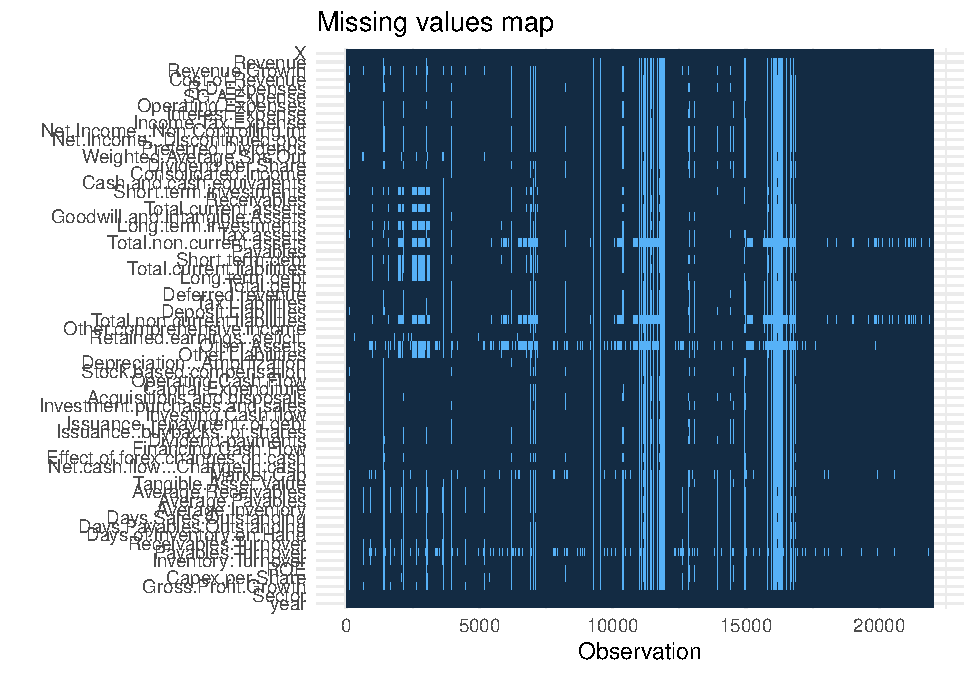
\includegraphics{stock_analysis_files/figure-latex/missing values-1.pdf}
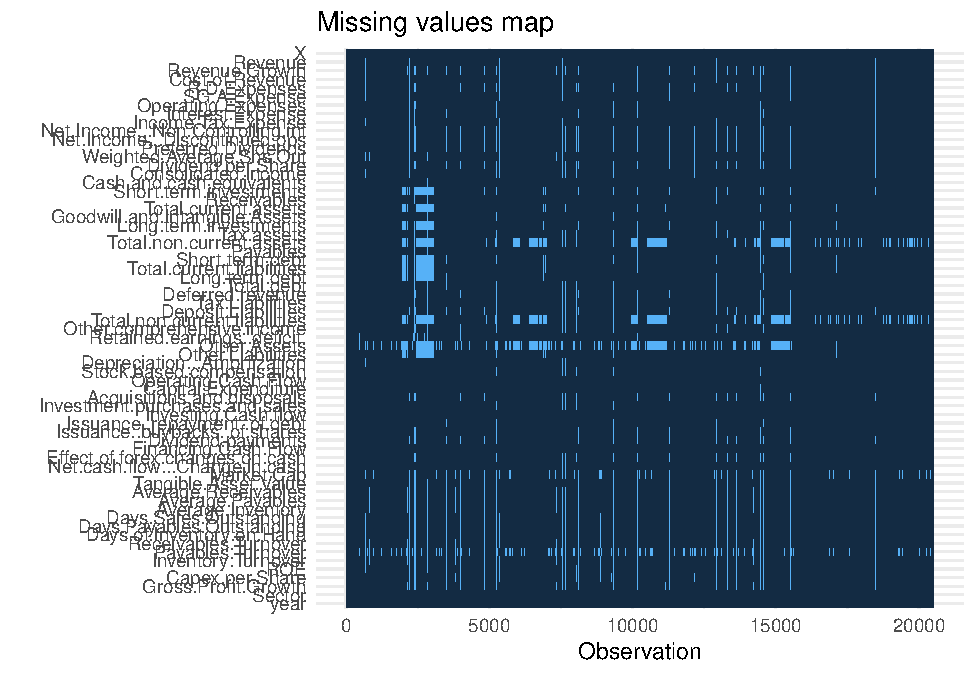
\includegraphics{stock_analysis_files/figure-latex/missing values-2.pdf}

To account for missing values, we chose to use the CART (Classification
and Regression Trees) method of imputation
(\hyperref[sec:fig2]{Figure 2}). Blue represents the distribution of the
original data, while red represents the distribution of imputed data.
After imputation, 4 columns still have missing values.

\begin{verbatim}
##       X                Revenue           Revenue.Growth    
##  Length:20526       Min.   :-6.276e+08   Min.   :   -6.87  
##  Class :character   1st Qu.: 6.567e+07   1st Qu.:   -0.01  
##  Mode  :character   Median : 4.684e+08   Median :    0.06  
##                     Mean   : 4.883e+09   Mean   :    5.72  
##                     3rd Qu.: 2.367e+09   3rd Qu.:    0.18  
##                     Max.   : 5.003e+11   Max.   :42138.66  
##  Cost.of.Revenue       R.D.Expenses         SG.A.Expense       
##  Min.   :-2.987e+09   Min.   :-1.098e+08   Min.   :-1.402e+08  
##  1st Qu.: 3.380e+06   1st Qu.: 0.000e+00   1st Qu.: 1.778e+07  
##  Median : 1.519e+08   Median : 0.000e+00   Median : 8.048e+07  
##  Mean   : 2.942e+09   Mean   : 1.037e+08   Mean   : 8.508e+08  
##  3rd Qu.: 1.171e+09   3rd Qu.: 1.235e+07   3rd Qu.: 3.698e+08  
##  Max.   : 3.771e+11   Max.   : 2.884e+10   Max.   : 1.065e+11  
##  Operating.Expenses   Interest.Expense     Income.Tax.Expense  
##  Min.   :-5.496e+09   Min.   :-1.711e+09   Min.   :-7.380e+11  
##  1st Qu.: 3.582e+07   1st Qu.: 0.000e+00   1st Qu.: 0.000e+00  
##  Median : 1.565e+08   Median : 3.684e+06   Median : 3.374e+06  
##  Mean   : 1.354e+09   Mean   : 9.349e+07   Mean   : 1.242e+08  
##  3rd Qu.: 6.233e+08   3rd Qu.: 4.994e+07   3rd Qu.: 4.443e+07  
##  Max.   : 1.065e+11   Max.   : 1.845e+10   Max.   : 8.490e+11  
##  Net.Income...Non.Controlling.int Net.Income...Discontinued.ops
##  Min.   :-1.587e+09               Min.   :-1.591e+10           
##  1st Qu.: 0.000e+00               1st Qu.: 0.000e+00           
##  Median : 0.000e+00               Median : 0.000e+00           
##  Mean   : 1.343e+07               Mean   :-4.430e+06           
##  3rd Qu.: 0.000e+00               3rd Qu.: 0.000e+00           
##  Max.   : 6.431e+09               Max.   : 8.368e+09           
##  Preferred.Dividends  Weighted.Average.Shs.Out Dividend.per.Share 
##  Min.   :-161000000   Min.   :0.000e+00        Min.   :    0.000  
##  1st Qu.:         0   1st Qu.:1.743e+07        1st Qu.:    0.000  
##  Median :         0   Median :4.421e+07        Median :    0.000  
##  Mean   :   4816894   Mean   :2.620e+08        Mean   :    1.197  
##  3rd Qu.:         0   3rd Qu.:1.196e+08        3rd Qu.:    0.720  
##  Max.   :2741588000   Max.   :1.113e+11        Max.   :10100.664  
##  Consolidated.Income  Cash.and.cash.equivalents Short.term.investments
##  Min.   :-2.244e+10   Min.   :0.000e+00         Min.   :0.000e+00     
##  1st Qu.:-9.438e+06   1st Qu.:1.809e+07         1st Qu.:0.000e+00     
##  Median : 1.950e+07   Median :7.410e+07         Median :0.000e+00     
##  Mean   : 3.798e+08   Mean   :1.538e+09         Mean   :1.483e+09     
##  3rd Qu.: 1.643e+08   3rd Qu.:2.976e+08         3rd Qu.:1.800e+07     
##  Max.   : 5.953e+10   Max.   :5.123e+11         Max.   :8.000e+11     
##   Receivables        Total.current.assets Goodwill.and.Intangible.Assets
##  Min.   :0.000e+00   Min.   :0.000e+00    Min.   :0.000e+00             
##  1st Qu.:2.169e+06   1st Qu.:6.823e+07    1st Qu.:0.000e+00             
##  Median :4.472e+07   Median :2.822e+08    Median :3.743e+07             
##  Mean   :8.594e+08   Mean   :5.709e+09    Mean   :1.708e+09             
##  3rd Qu.:2.889e+08   3rd Qu.:1.234e+09    3rd Qu.:4.915e+08             
##  Max.   :1.624e+11   Max.   :1.181e+12    Max.   :2.931e+11             
##  Long.term.investments   Tax.assets           Payables         
##  Min.   :-8.000e+07    Min.   :0.000e+00   Min.   :-2.059e+10  
##  1st Qu.: 0.000e+00    1st Qu.:0.000e+00   1st Qu.: 2.801e+06  
##  Median : 0.000e+00    Median :0.000e+00   Median : 2.620e+07  
##  Mean   : 3.621e+09    Mean   :1.498e+08   Mean   : 8.274e+08  
##  3rd Qu.: 6.371e+07    3rd Qu.:1.566e+07   3rd Qu.: 1.820e+08  
##  Max.   : 9.970e+11    Max.   :4.262e+10   Max.   : 2.136e+11  
##  Short.term.debt      Total.current.liabilities Long.term.debt      
##  Min.   :-1.375e+09   Min.   :-2.108e+10        Min.   :-8.446e+09  
##  1st Qu.: 0.000e+00   1st Qu.: 2.838e+07        1st Qu.: 7.345e+05  
##  Median : 1.666e+06   Median : 1.810e+08        Median : 1.504e+08  
##  Mean   : 6.148e+08   Mean   : 8.541e+09        Mean   : 2.999e+09  
##  3rd Qu.: 4.003e+07   3rd Qu.: 1.040e+09        3rd Qu.: 1.285e+09  
##  Max.   : 2.192e+11   Max.   : 2.095e+12        Max.   : 7.330e+11  
##    Total.debt         Deposit.Liabilities Other.comprehensive.income
##  Min.   :-9.290e+09   Min.   :0.000e+00   Min.   :-9.478e+10        
##  1st Qu.: 5.916e+06   1st Qu.:0.000e+00   1st Qu.:-2.083e+07        
##  Median : 2.131e+08   Median :0.000e+00   Median :-2.335e+05        
##  Mean   : 4.158e+09   Mean   :4.917e+09   Mean   : 8.310e+10        
##  3rd Qu.: 1.486e+09   3rd Qu.:0.000e+00   3rd Qu.: 0.000e+00        
##  Max.   : 1.014e+12   Max.   :1.471e+12   Max.   : 1.709e+15        
##  Retained.earnings..deficit.  Other.Assets        Other.Liabilities   
##  Min.   :-2.800e+11          Min.   :-9.120e+11   Min.   :-9.923e+10  
##  1st Qu.:-1.190e+08          1st Qu.: 1.878e+06   1st Qu.: 7.704e+06  
##  Median : 2.056e+07          Median : 1.542e+07   Median : 6.580e+07  
##  Mean   : 2.005e+09          Mean   : 1.430e+09   Mean   : 7.223e+09  
##  3rd Qu.: 5.367e+08          3rd Qu.: 9.163e+07   3rd Qu.: 4.791e+08  
##  Max.   : 4.217e+11          Max.   : 6.010e+11   Max.   : 1.866e+12  
##  Depreciation...Amortization Stock.based.compensation Operating.Cash.Flow 
##  Min.   :-8.336e+07          Min.   :-137000000       Min.   :-3.180e+11  
##  1st Qu.: 2.046e+06          1st Qu.:    496050       1st Qu.: 1.018e+06  
##  Median : 2.086e+07          Median :   3811000       Median : 5.854e+07  
##  Mean   : 3.358e+08          Mean   :  31793457       Mean   : 8.704e+08  
##  3rd Qu.: 1.256e+08          3rd Qu.:  14953500       3rd Qu.: 3.394e+08  
##  Max.   : 7.510e+11          Max.   :9353000000       Max.   : 9.600e+11  
##  Capital.Expenditure  Acquisitions.and.disposals Investment.purchases.and.sales
##  Min.   :-9.662e+10   Min.   :-5.100e+10         Min.   :-1.930e+11            
##  1st Qu.:-1.291e+08   1st Qu.:-1.153e+07         1st Qu.:-1.017e+07            
##  Median :-1.700e+07   Median : 0.000e+00         Median : 0.000e+00            
##  Mean   :-3.608e+08   Mean   :-1.030e+08         Mean   :-1.764e+08            
##  3rd Qu.:-1.344e+06   3rd Qu.: 0.000e+00         3rd Qu.: 0.000e+00            
##  Max.   : 5.823e+09   Max.   : 6.987e+10         Max.   : 1.499e+11            
##  Investing.Cash.flow  Issuance..repayment..of.debt
##  Min.   :-1.980e+11   Min.   :-8.488e+10          
##  1st Qu.:-2.887e+08   1st Qu.:-1.045e+07          
##  Median :-4.875e+07   Median : 0.000e+00          
##  Mean   :-6.591e+08   Mean   : 6.767e+07          
##  3rd Qu.:-1.848e+06   3rd Qu.: 4.738e+07          
##  Max.   : 1.446e+11   Max.   : 6.268e+10          
##  Issuance..buybacks..of.shares Dividend.payments    Financing.Cash.Flow 
##  Min.   :-7.207e+10            Min.   :-1.603e+10   Min.   :-1.875e+11  
##  1st Qu.:-8.241e+06            1st Qu.:-5.092e+07   1st Qu.:-7.786e+07  
##  Median : 0.000e+00            Median : 0.000e+00   Median : 0.000e+00  
##  Mean   :-1.140e+08            Mean   :-1.854e+08   Mean   :-6.441e+07  
##  3rd Qu.: 6.221e+06            3rd Qu.: 0.000e+00   3rd Qu.: 5.758e+07  
##  Max.   : 1.444e+11            Max.   : 0.000e+00   Max.   : 2.260e+11  
##  Effect.of.forex.changes.on.cash Net.cash.flow...Change.in.cash
##  Min.   :-1.000e+12              Min.   :-1.525e+11            
##  1st Qu.:-2.668e+05              1st Qu.:-1.689e+07            
##  Median : 0.000e+00              Median : 7.057e+05            
##  Mean   :-6.421e+07              Mean   : 7.016e+07            
##  3rd Qu.: 0.000e+00              3rd Qu.: 2.900e+07            
##  Max.   : 9.993e+09              Max.   : 4.050e+11            
##    Market.Cap        Tangible.Asset.Value Average.Receivables
##  Min.   :0.000e+00   Min.   :-2.422e+10   Min.   :0.000e+00  
##  1st Qu.:1.970e+08   1st Qu.: 1.681e+08   1st Qu.:2.378e+06  
##  Median :9.249e+08   Median : 9.063e+08   Median :4.341e+07  
##  Mean   :8.305e+09   Mean   : 1.611e+10   Mean   :8.522e+08  
##  3rd Qu.:4.029e+09   3rd Qu.: 4.047e+09   3rd Qu.:2.831e+08  
##  Max.   :1.098e+12   Max.   : 2.568e+12   Max.   :1.614e+11  
##  Average.Payables     Average.Inventory   Days.Sales.Outstanding
##  Min.   :-2.037e+10   Min.   :0.000e+00   Min.   :-165044.9     
##  1st Qu.: 2.911e+06   1st Qu.:0.000e+00   1st Qu.:     10.6     
##  Median : 2.619e+07   Median :1.693e+06   Median :     45.4     
##  Mean   : 9.308e+08   Mean   :4.189e+08   Mean   :    197.2     
##  3rd Qu.: 1.783e+08   3rd Qu.:1.009e+08   3rd Qu.:     72.3     
##  Max.   : 7.124e+11   Max.   :4.560e+11   Max.   :1504680.2     
##  Days.Payables.Outstanding Days.of.Inventory.on.Hand Receivables.Turnover
##  Min.   :-207232.5         Min.   :-5182867          Min.   :   -27.99   
##  1st Qu.:     10.3         1st Qu.:     -70          1st Qu.:     2.70   
##  Median :     26.8         Median :      -5          Median :     5.96   
##  Mean   :    404.2         Mean   :    -650          Mean   :    44.53   
##  3rd Qu.:     55.7         3rd Qu.:       0          3rd Qu.:     9.89   
##  Max.   :1043413.3         Max.   :     976          Max.   :164428.50   
##  Payables.Turnover  Inventory.Turnover      ROE           Capex.per.Share    
##  Min.   : -41.096   Min.   :    0.00   Min.   :  -34772   Min.   :-73354000  
##  1st Qu.:   0.784   1st Qu.:    0.00   1st Qu.:       0   1st Qu.:       -2  
##  Median :   2.543   Median :    3.18   Median :       0   Median :        0  
##  Mean   :   7.394   Mean   :   33.30   Mean   :    1583   Mean   :   -19086  
##  3rd Qu.:   4.913   3rd Qu.:   10.63   3rd Qu.:       0   3rd Qu.:        0  
##  Max.   :8650.316   Max.   :95827.71   Max.   :11141142   Max.   :  1255873  
##  Gross.Profit.Growth    Sector            year     
##  Min.   : -5536.5    Length:20526       2014:3758  
##  1st Qu.:     0.0    Class :character   2015:3976  
##  Median :     0.1    Mode  :character   2016:4210  
##  Mean   :    19.6                       2017:4343  
##  3rd Qu.:     0.2                       2018:4239  
##  Max.   :336767.8
\end{verbatim}

\hypertarget{correlation-plot}{%
\subsection{Correlation Plot}\label{correlation-plot}}

There are 62 columns after we finished data cleaning, and we want to
select the important features to do modeling. We performed a correlation
analysis based on Pearson's coefficient between each numeric predictor
first. We considered a correlation \textgreater{} 0.5, with p
\textless{} 0.05 as a significant correlation.
\hyperref[sec:fig3]{Figure 3} demonstrates significant correlation
between many of our predictor variables. However, due to the large
amount of variables, the correlation plot is really hard to read if we
try to plot all the variables, therefore, we tried to filtered the
correlation plot. We only kept the variables has positive correlation
with a value greater than 0.8.

\begin{center}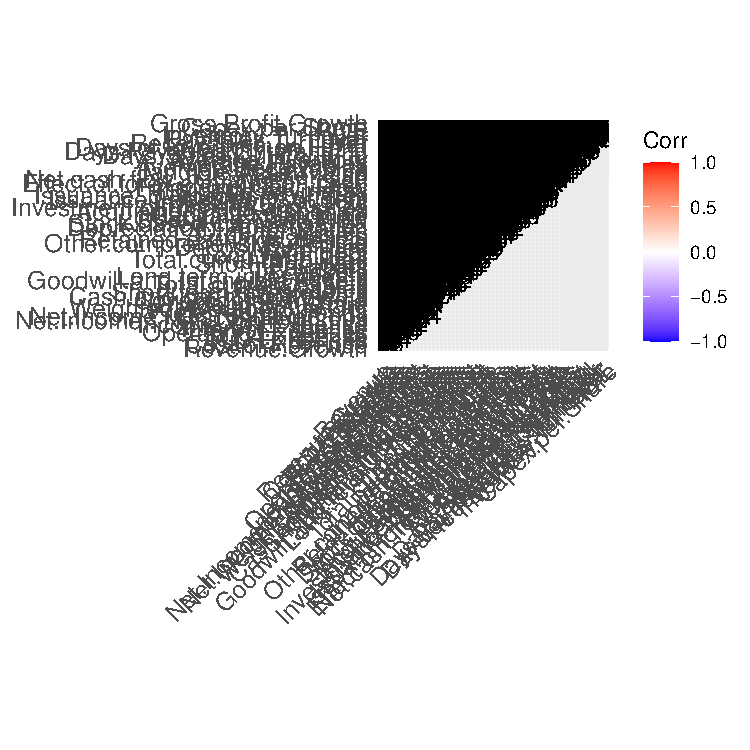
\includegraphics{stock_analysis_files/figure-latex/corrplot-1} \end{center}

\begin{verbatim}
##                      rowname                  variable correlation
## 1            Cost.of.Revenue                   Revenue   0.9529257
## 2         Operating.Expenses              SG.A.Expense   0.8649144
## 3       Total.current.assets Cash.and.cash.equivalents   0.8144814
## 4  Total.current.liabilities Cash.and.cash.equivalents   0.8693025
## 5        Deposit.Liabilities Cash.and.cash.equivalents   0.8613017
## 6          Other.Liabilities Cash.and.cash.equivalents   0.8658095
## 7       Tangible.Asset.Value Cash.and.cash.equivalents   0.8507838
## 8        Average.Receivables               Receivables   0.9754628
## 9  Total.current.liabilities      Total.current.assets   0.8852829
## 10                Total.debt      Total.current.assets   0.8465258
## 11         Other.Liabilities      Total.current.assets   0.8595369
## 12      Tangible.Asset.Value      Total.current.assets   0.8866186
## 13                Total.debt Total.current.liabilities   0.8169391
## 14       Deposit.Liabilities Total.current.liabilities   0.9418235
## 15         Other.Liabilities Total.current.liabilities   0.9889940
## 16      Tangible.Asset.Value Total.current.liabilities   0.9566535
## 17      Tangible.Asset.Value                Total.debt   0.8338607
## 18         Other.Liabilities       Deposit.Liabilities   0.9484187
## 19      Tangible.Asset.Value       Deposit.Liabilities   0.8932697
## 20      Tangible.Asset.Value         Other.Liabilities   0.9426275
## 21 Days.of.Inventory.on.Hand         Average.Inventory  -0.9128818
\end{verbatim}

\begin{verbatim}
## [1] "Cost.of.Revenue"           "Operating.Expenses"       
## [3] "Tangible.Asset.Value"      "Average.Receivables"      
## [5] "Days.of.Inventory.on.Hand"
\end{verbatim}

\begin{center}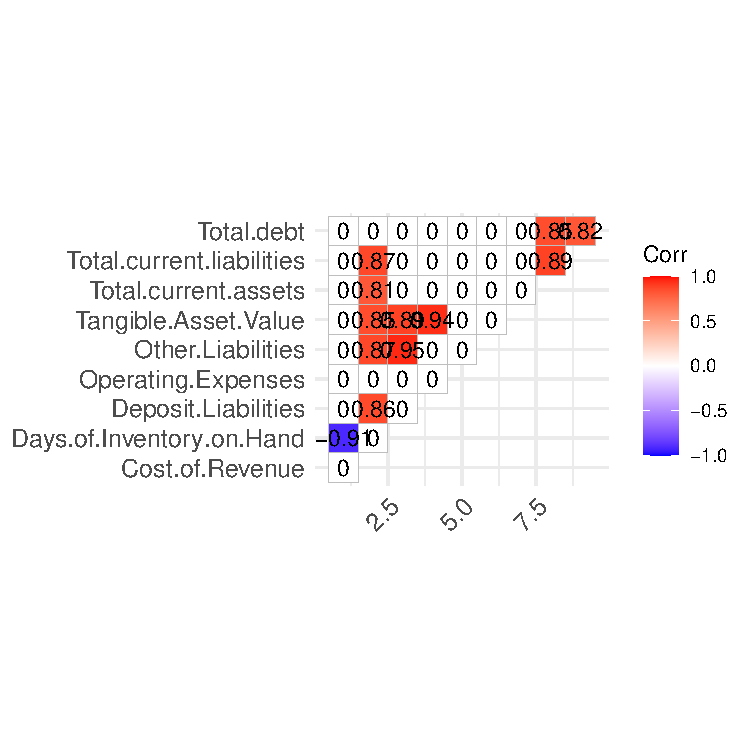
\includegraphics{stock_analysis_files/figure-latex/corrplot-2} \end{center}

\hypertarget{data-distribution}{%
\subsection{Data Distribution}\label{data-distribution}}

we then performed the distribution plot for all the columns to check the
data distribution, to oberseve the means, and check is there any
outliers.

\begin{center}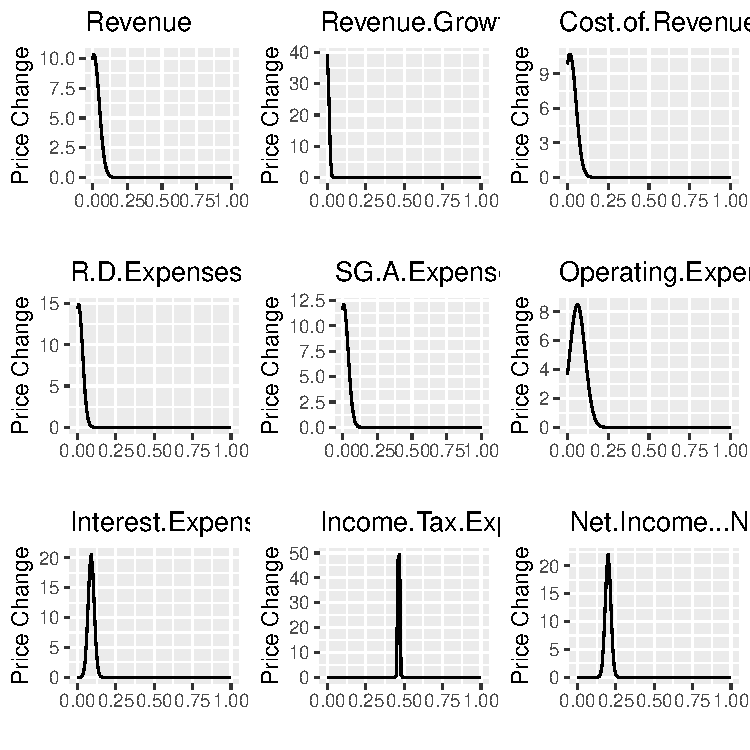
\includegraphics{stock_analysis_files/figure-latex/data normal distribution plot1-1} \end{center}

\begin{center}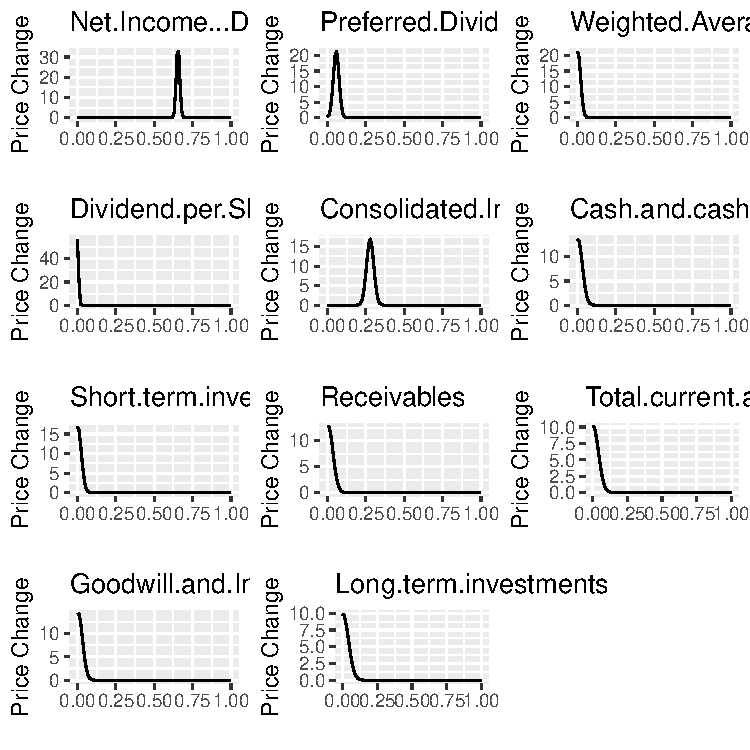
\includegraphics{stock_analysis_files/figure-latex/data normal distribution plot2-1} \end{center}

\begin{center}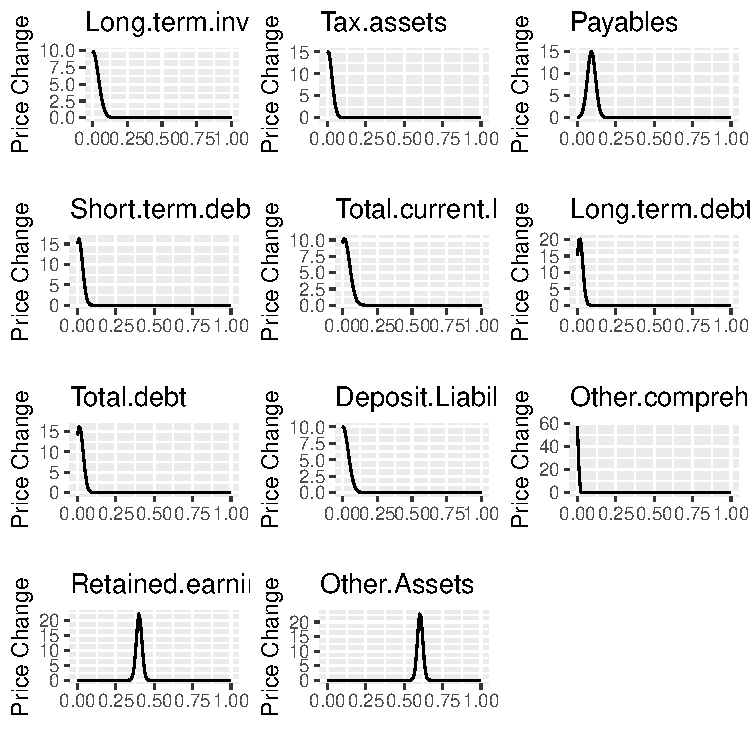
\includegraphics{stock_analysis_files/figure-latex/data normal distribution plot3-1} \end{center}

\begin{center}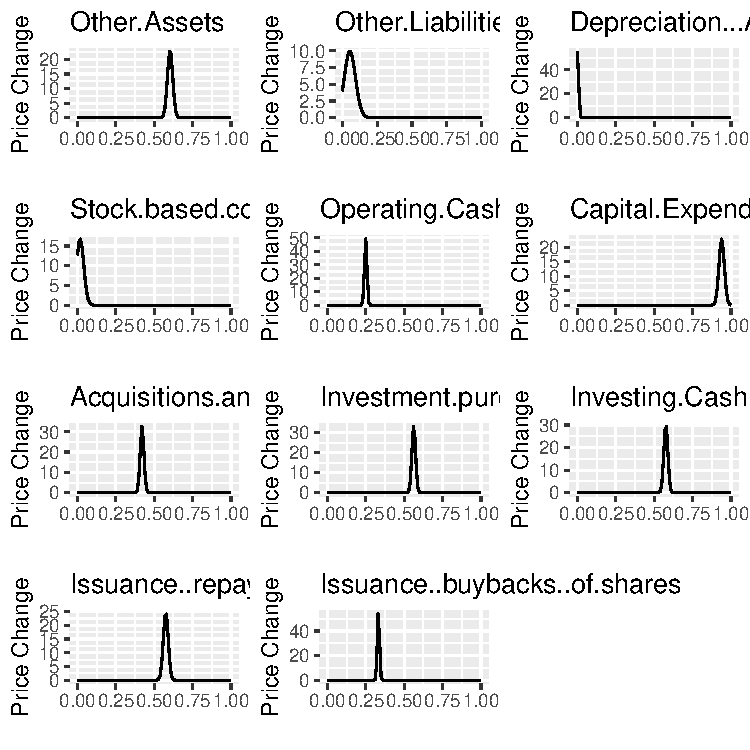
\includegraphics{stock_analysis_files/figure-latex/data normal distribution plot4-1} \end{center}

\begin{center}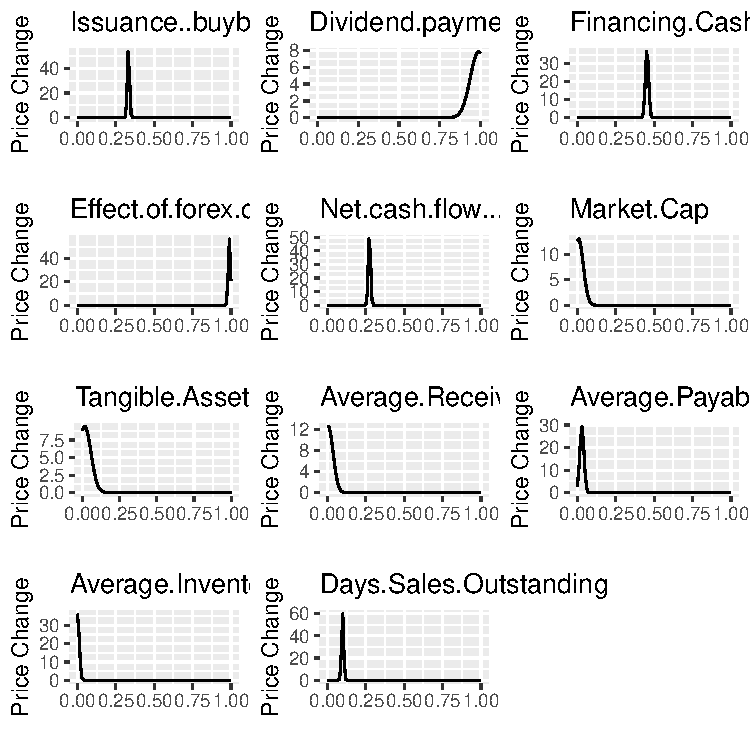
\includegraphics{stock_analysis_files/figure-latex/data normal distribution plot5-1} \end{center}

\begin{center}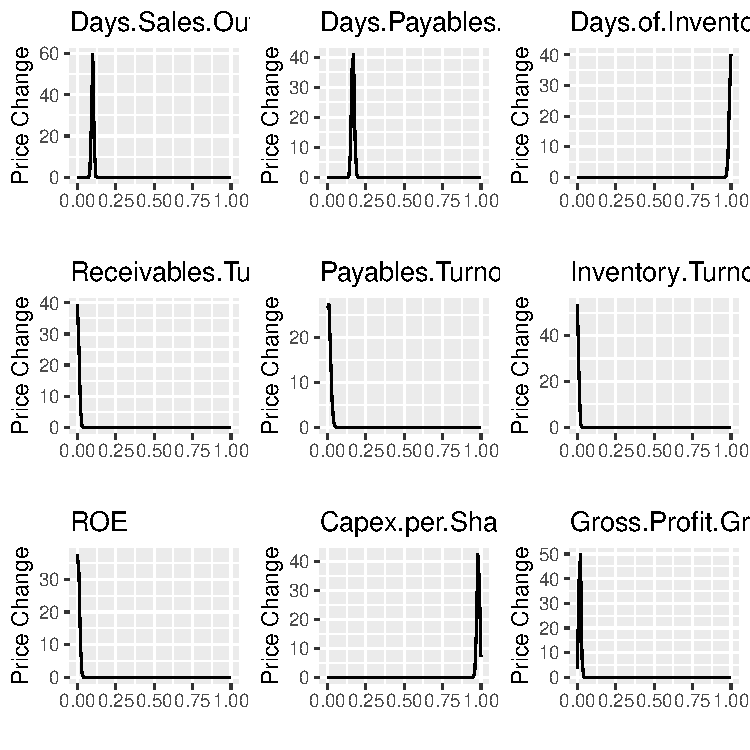
\includegraphics{stock_analysis_files/figure-latex/data normal distribution plot6-1} \end{center}

\hypertarget{feature-selection-1}{%
\subsection{Feature Selection}\label{feature-selection-1}}

In order to do our feature selection, we ran a decision tree model to do
a variable importance analysis.

\begin{Shaded}
\begin{Highlighting}[]
\CommentTok{#decision_tree_model <-readRDS('decision_tree_model.rds')}
\CommentTok{#print(decision_tree_model)}
\CommentTok{#dTreeImp <- varImp(decision_tree_model, scale = FALSE)}
\CommentTok{#plot(dTreeImp, top = 10)}
\CommentTok{#invisible(model_importance <- summary(decision_tree_model$finalModel))}
\end{Highlighting}
\end{Shaded}

We also did some data visualization for our final data set which we will
use for modeling.

Correlation plot for the final dataset

\begin{center}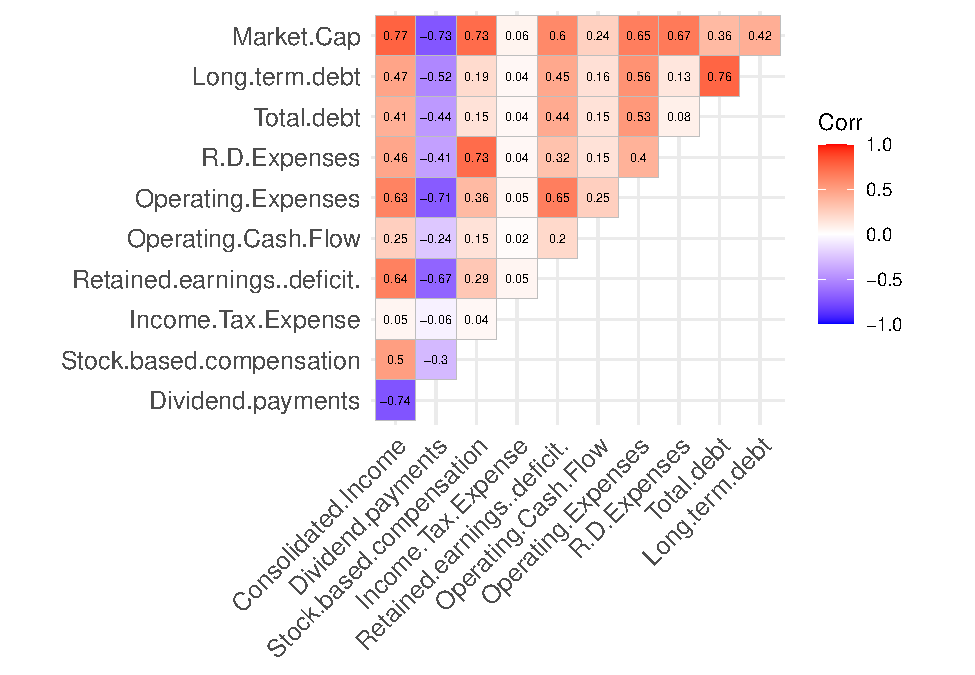
\includegraphics{stock_analysis_files/figure-latex/correlation plot 2-1} \end{center}

\hypertarget{principle-component-analysis-1}{%
\subsection{Principle Component
Analysis}\label{principle-component-analysis-1}}

We performed PCA to reduce the dimensionality of our feature dataset.
The Scree plot shows the overall variance explained by each principle
component. The top 5 dimensions explained approximately 90\% of the
total variance within the data. Individual datapoints involving large
technology companies (Google, Apple, Amazon) had high contributions to
the overall variance. R\&D Expenses and Stock-based compensation were
two variables with high contribution to variance, while Income Tax
Expense and Operating Cash Flow had more negligible contribution.

\begin{figure}

{\centering 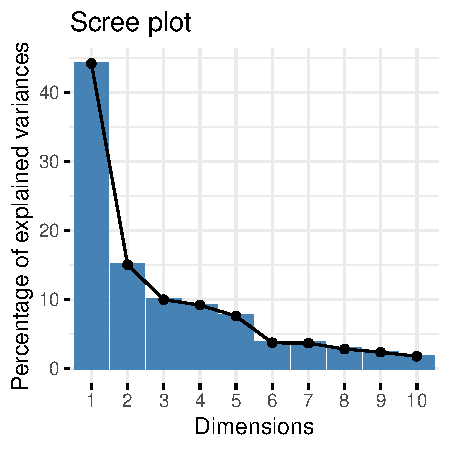
\includegraphics{stock_analysis_files/figure-latex/scree-1} 

}

\caption{Scree plot}\label{fig:scree}
\end{figure}

\begin{figure}

{\centering 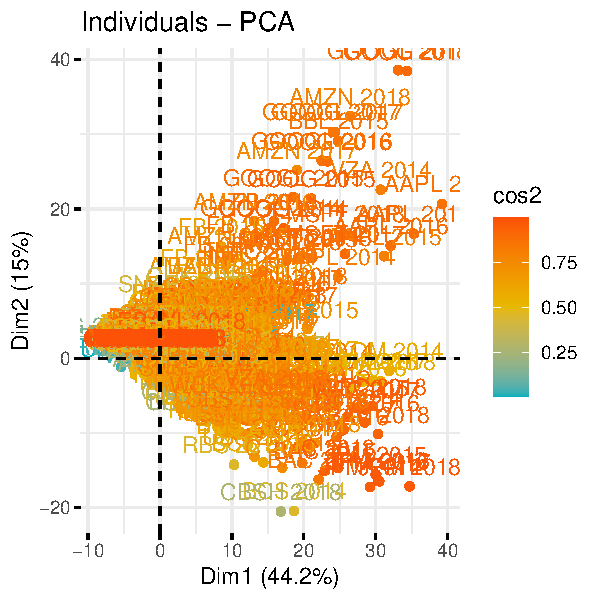
\includegraphics{stock_analysis_files/figure-latex/PCAind-1} 

}

\caption{Effect of Individual points - PCA}\label{fig:PCAind}
\end{figure}
\begin{figure}

{\centering 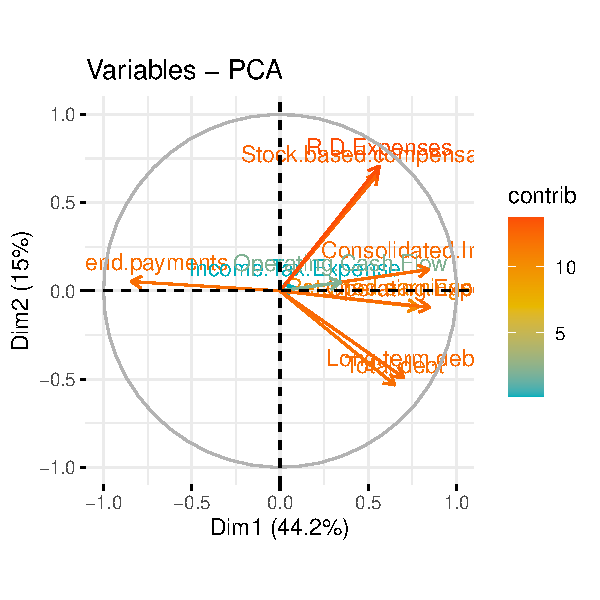
\includegraphics{stock_analysis_files/figure-latex/PCAvar-1} 

}

\caption{Effect of Variables - PCA}\label{fig:PCAvar}
\end{figure}

\hypertarget{k-means-clustering}{%
\subsection{K Means Clustering}\label{k-means-clustering}}

The `elbow method' was first performed to determine an optimal number of
k clusters. However, there was no significant drop in within-cluster sum
of squares with k besides k=2. As two clusters did not provide much
discrimination for our observations, we instead used k=4 as the final
number of clusters.

\begin{figure}
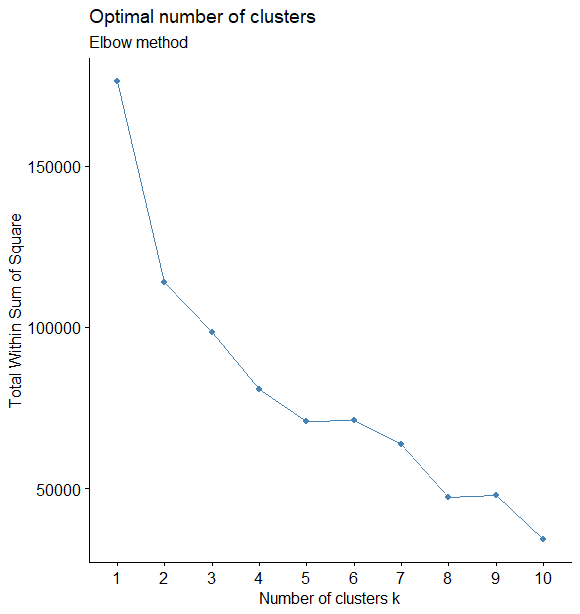
\includegraphics[width=0.7\linewidth,height=0.5\textheight]{unsupervised_elbow} \caption{Elbow method}\label{fig:elbow}
\end{figure}

The following figure displays our datapoints in a 2-D space based on 4
clusters. (will show the cluster plots and more by tomorrow evening)

\begin{figure}
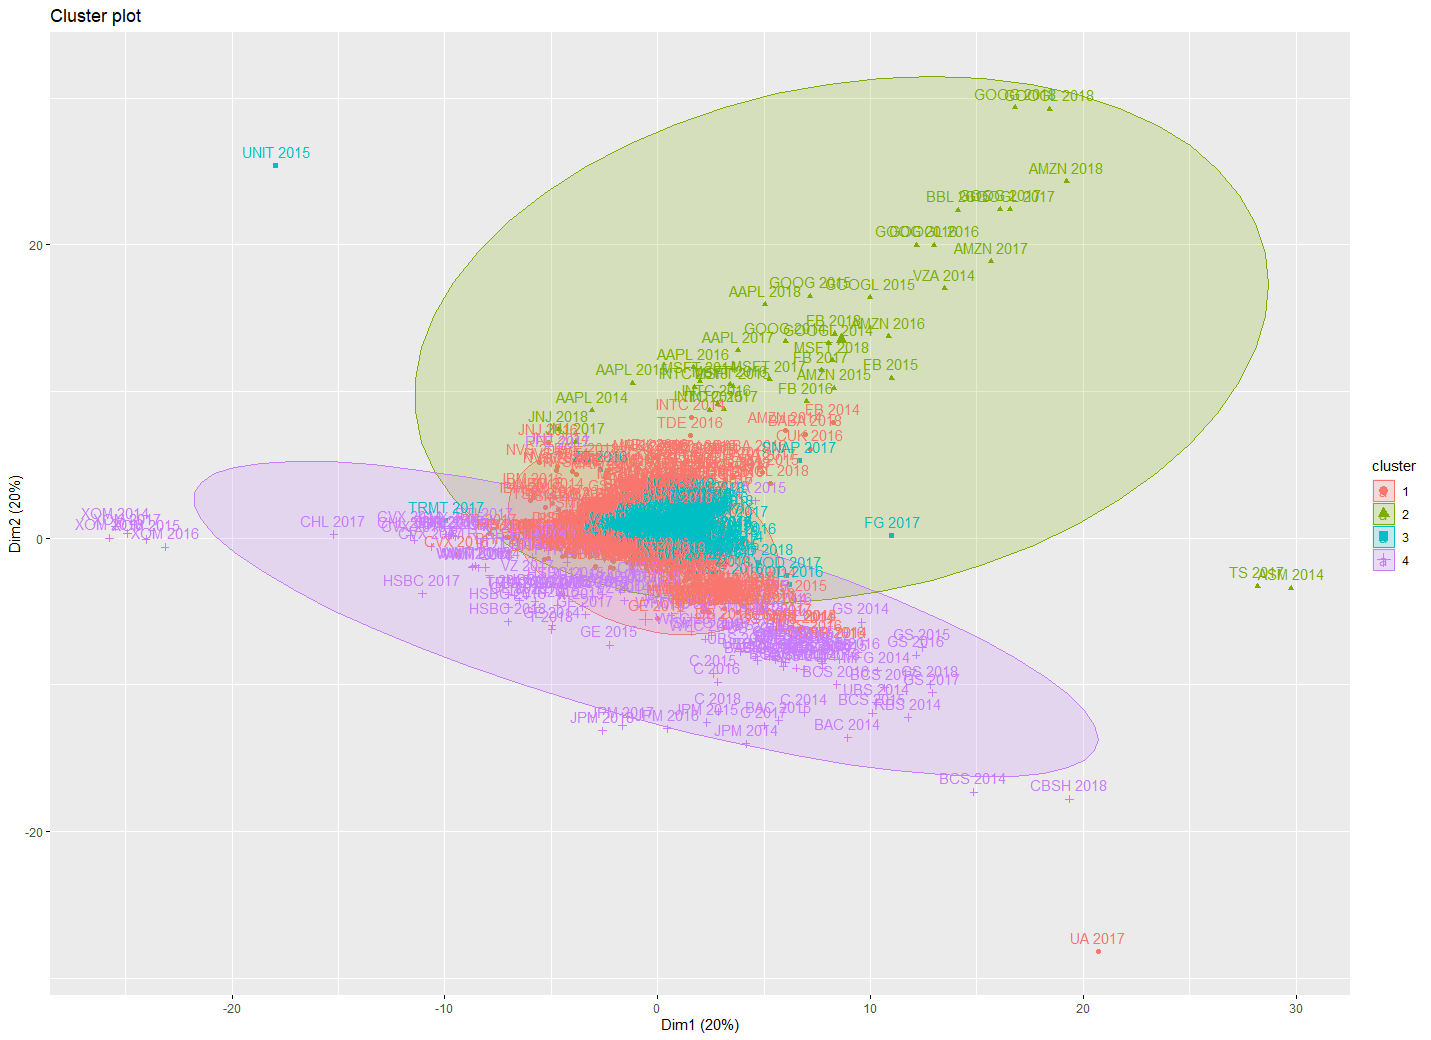
\includegraphics[width=1\linewidth,height=0.7\textheight]{cluster_image} \caption{K means clustering, k = 4}\label{fig:cluster}
\end{figure}

\hypertarget{modeling}{%
\subsection{Modeling}\label{modeling}}

The k-fold cross-validation method evaluates the model performance on
different subsets of the training data calculates the average prediction
error rate. We used k = 10 for our project,and this method was used
instead of the simple train-test-split as it gives a more valid
estimation of model effectiveness.

\hypertarget{random-forest}{%
\paragraph{\texorpdfstring{\textbf{Random Forest}\\
}{Random Forest }}\label{random-forest}}

\hypertarget{xgboost}{%
\paragraph{\texorpdfstring{\textbf{XGBoost}\\
}{XGBoost }}\label{xgboost}}

For the XGBoost model, we used nrounds, eta, max\_depth as tuning
parameters to increase the accuarcy of the final model and reduce
errors. The model used tuning parameter `subsample' as a constant at a
value of 0.8, and RMSE was used to select the optimal model using the
smallest value. The final values used for the model were nrounds = 200,
max\_depth = 6, eta = 0.1, gamma = 0, colsample\_bytree = 0.5,
min\_child\_weight = 1 and subsample = 0.8.

\begin{verbatim}
## [15:59:17] WARNING: amalgamation/../src/objective/regression_obj.cu:174: reg:linear is now deprecated in favor of reg:squarederror.
\end{verbatim}

\begin{center}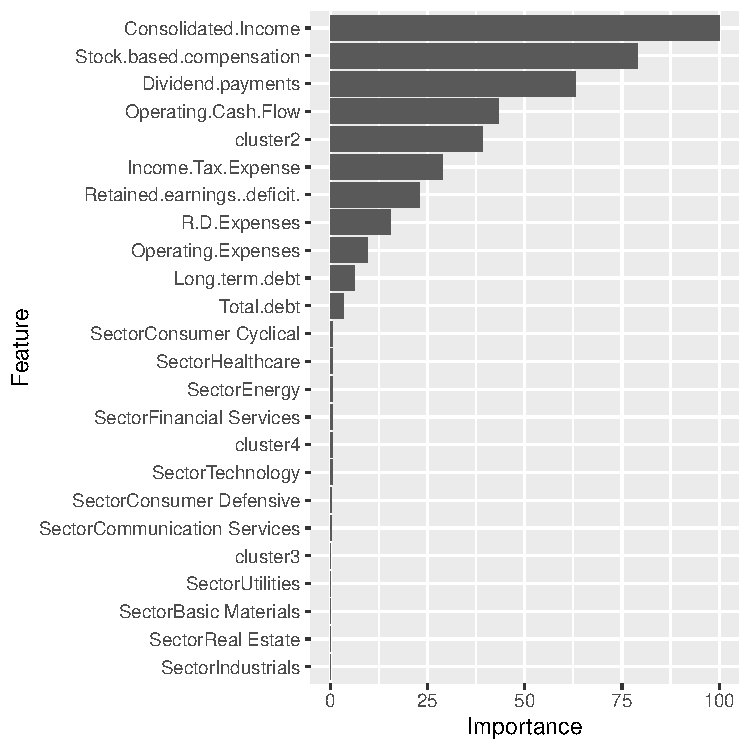
\includegraphics{stock_analysis_files/figure-latex/XGBoost-1} \end{center}

\begin{center}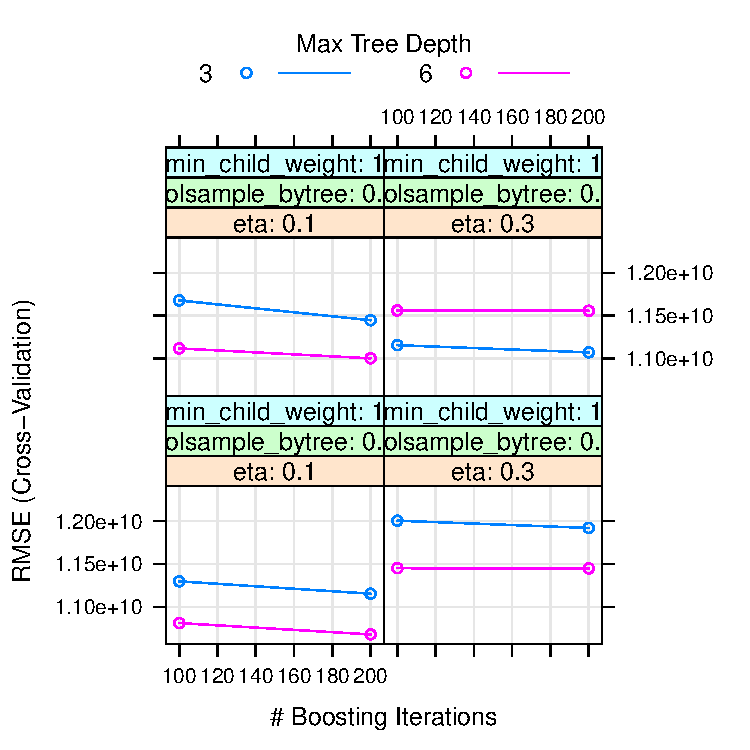
\includegraphics{stock_analysis_files/figure-latex/XGBoost-2} \end{center}

\begin{center}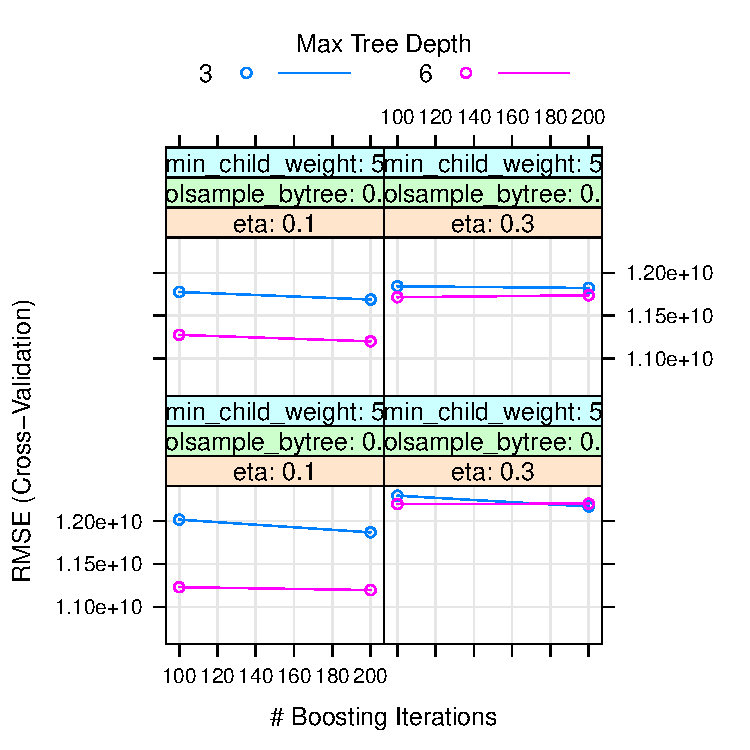
\includegraphics{stock_analysis_files/figure-latex/XGBoost-3} \end{center}

\hypertarget{lasso-regression}{%
\paragraph{\texorpdfstring{\textbf{Lasso Regression}\\
}{Lasso Regression }}\label{lasso-regression}}

For the lasso regression model, RMSE was used to select the optimal
model using the smallest value. The final value used for the model was
fraction = 0.9.

\begin{center}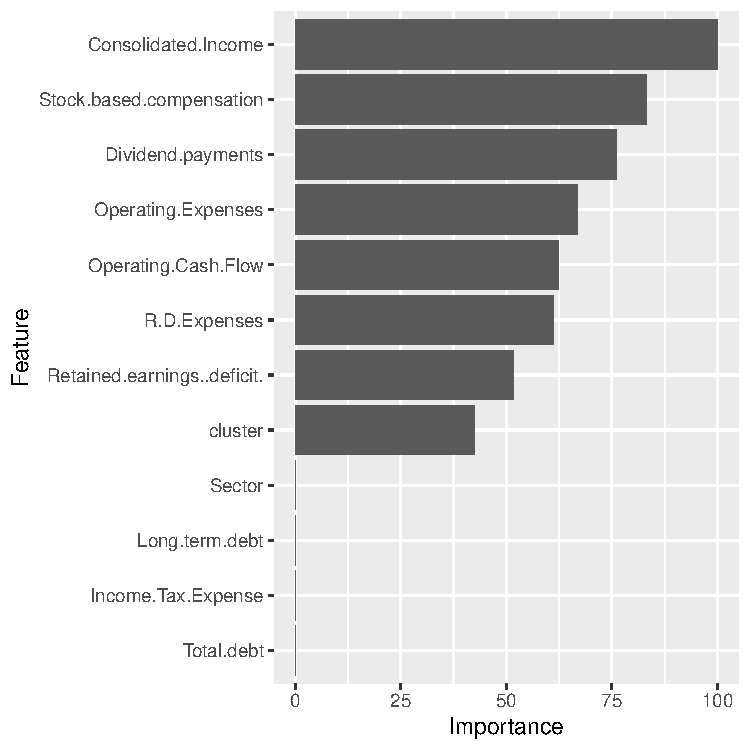
\includegraphics{stock_analysis_files/figure-latex/Lasso regression-1} \end{center}

\hypertarget{gradient-boosting}{%
\paragraph{\texorpdfstring{\textbf{Gradient Boosting}\\
}{Gradient Boosting }}\label{gradient-boosting}}

The gradient boosting model was tuned by several different parameters.
The final values used for the model were n.trees = 600,
interaction.depth = 9, shrinkage = 0.1 and n.minobsinnode = 20

\begin{center}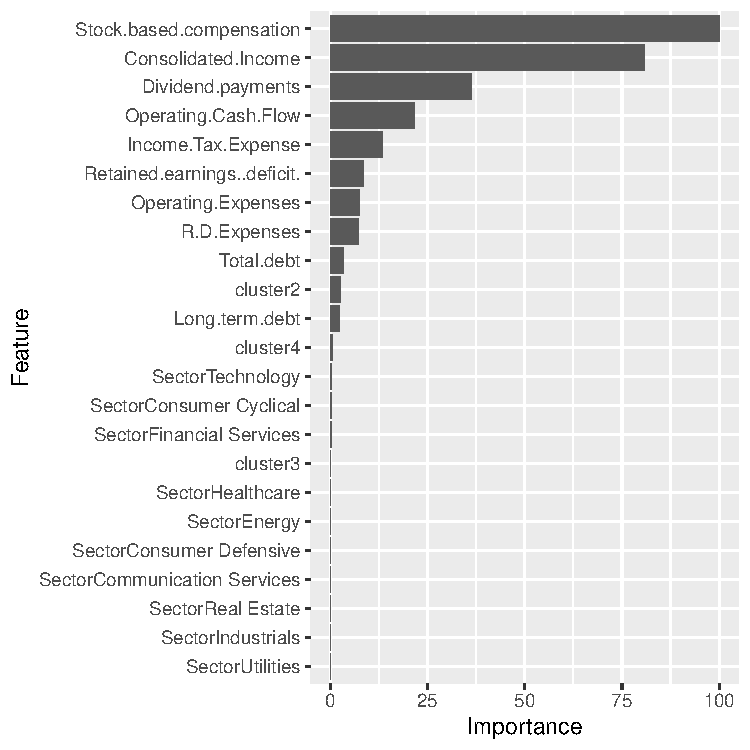
\includegraphics{stock_analysis_files/figure-latex/gradient boosting-1} \end{center}

\#\#\#Model Selection All models found \(nmnmb\) and \(hghh\) to be
important predictors of Market.Cap. Mean Absolute Error (MAE) tells the
average error of the variable we want to predict. Root Mean-Squared
Error (RMSE) is similar with MAE but it is more useful when we are
interested in fewer larger errors over many small errors. Overall, we
prioritize model stability and thus prioritized RMSE over MAE. \(R^2\)
computes how much better the regression fits the data than the mean
line, which gives an overall score.For predicting market cap, we desired
a model with the lowest RMSE and MAE to keep the high accuracy of
prediction. The XGBoost model had the highest \(R^2\) as well as the
lowest RMSE and MAE, thus, it was chosen for deployment.

\begin{longtable}[]{@{}llrl@{}}
\caption{Model Accuracy}\tabularnewline
\toprule
model & RMSE & R2 & MAE\tabularnewline
\midrule
\endfirsthead
\toprule
model & RMSE & R2 & MAE\tabularnewline
\midrule
\endhead
random\_forest & 2.75e+05 & 0.81 & 1.36e+05\tabularnewline
extreme\_gradient\_boosting & 1.08e+10 & 0.90 & 2.70e+09\tabularnewline
Lasso\_Regression & 1.45e+10 & 0.82 & 3.75e+09\tabularnewline
gradient\_boosting & 1.18e+10 & 0.88 & 2.92e+09\tabularnewline
\bottomrule
\end{longtable}

\hypertarget{discussion}{%
\section{Discussion}\label{discussion}}





\newpage
\singlespacing 
\end{document}
